\def\scaledim{0.44} 
\chapter{ROOT CERN}
ROOT è un framework sviluppato al CERN per l'analisi dati. È utilizzato per plottare (disegnare) dati su grafici, visualizzare istogrammi, fittare dati, ecc\ldots

Essenzialmente è una libreria che, una volta inclusa, permette al nostro programma di rappresentare graficamente numeri e dati, oltre ad essere dotata di diverse altre funzioni. Per sapere come installare ROOT, prova a leggere l'appendice \ref{instroot}.

La figura \ref{root1}, ad esempio, è realizzata con ROOT: è un plot di dati sperimentali raccolti da un rivelatore di raggi gamma. In poche parole, rappresenta lo spettro di radiazioni gamma emesse da una sorgente di radio 226: con ROOT possiamo scrivere programmi in \verb|C++| che producono output di questo tipo.
\begin{figure} [ht]
	\centering
	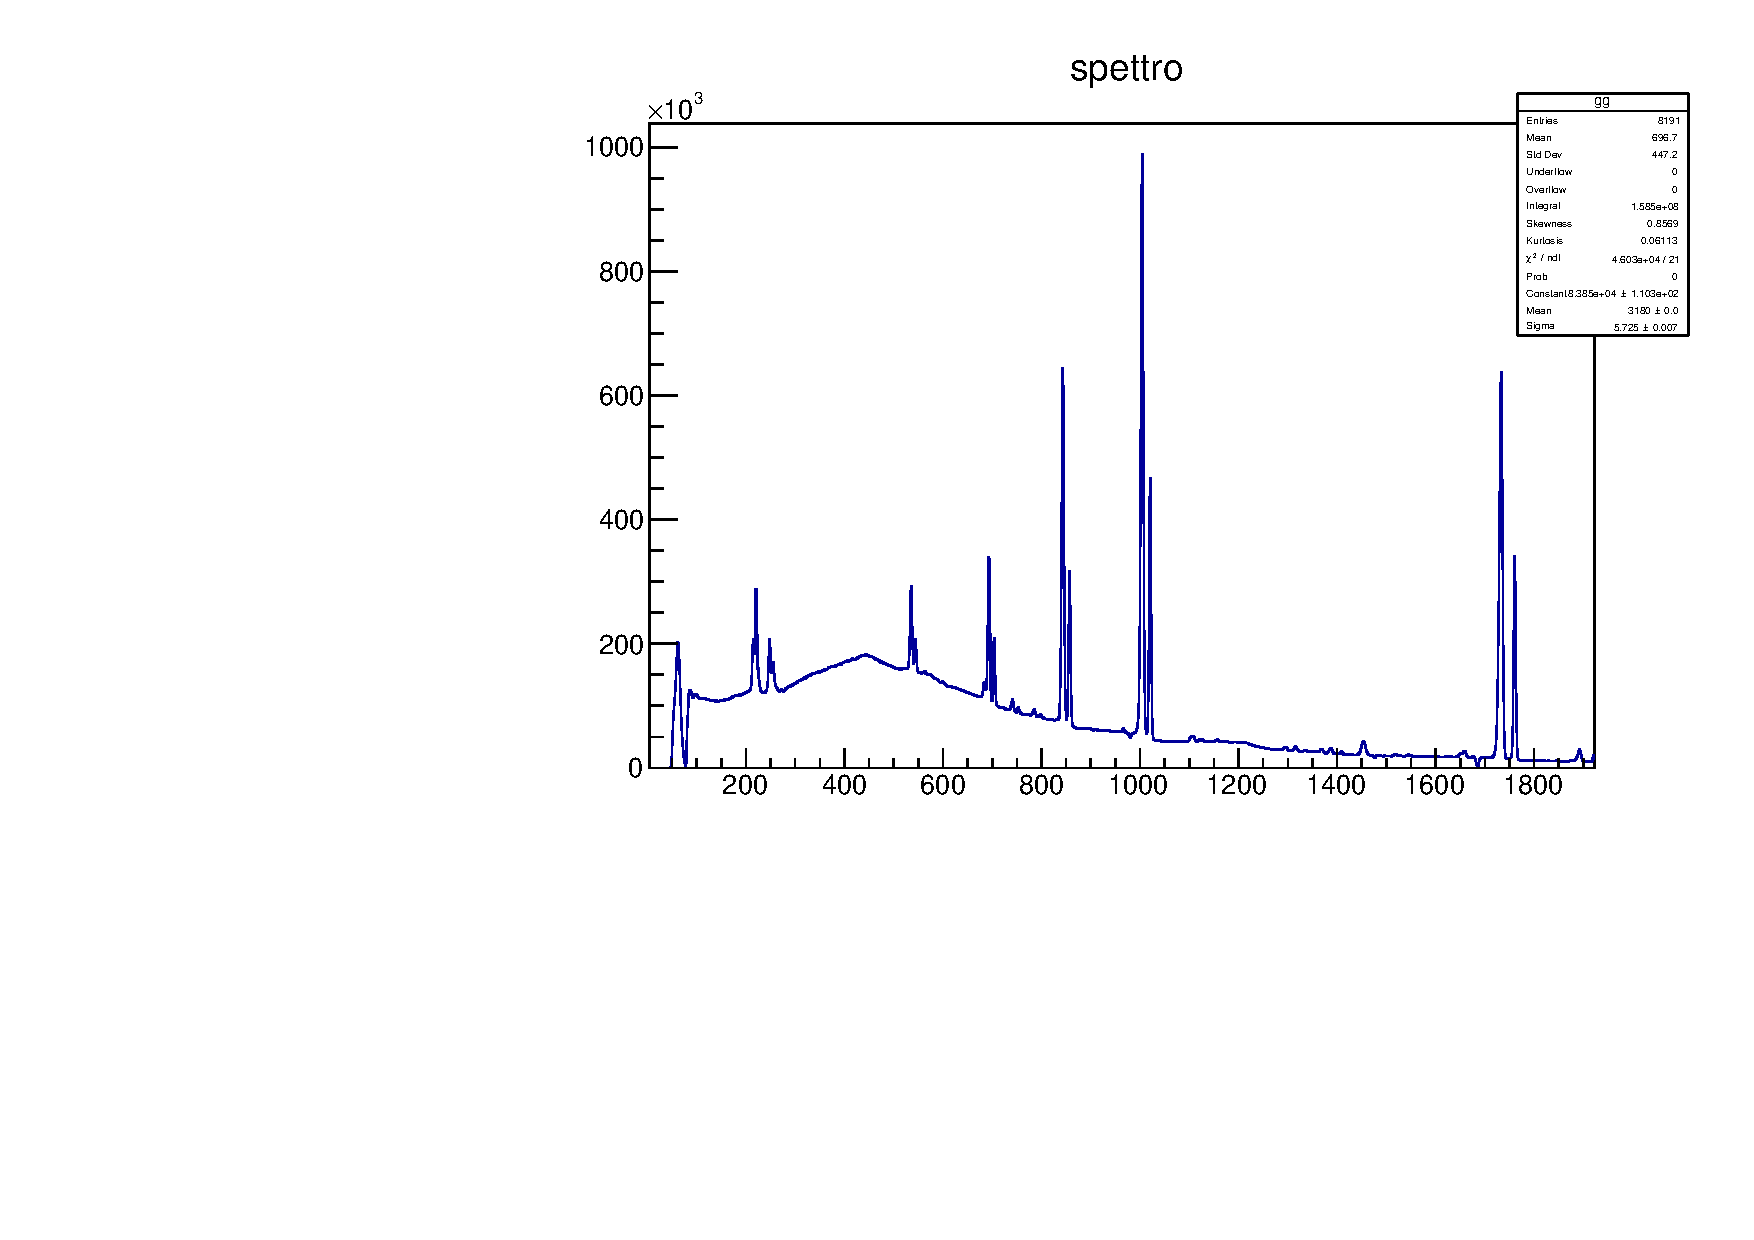
\includegraphics[scale=\scaledim]{Immagini/root1.pdf}  
	\caption{Radio 226}
	\label{root1}
\end{figure}


Questo capitolo sarà decisamente ``hands on'': c'è poco da capire, semplicemente dobbiamo imparare ad usare una libreria scritta da qualcun altro.
\section{Librerie da includere, flag di compilazione, TApplication e TCanvas}
Per poter usare ROOT, dobbiamo includere le librerie necessarie per avere a disposizione alcuni strumenti nel nostro codice. 

Due liberie che non possono mai mancare sono ``\verb|TApplication.h|'' e ``\verb|TCanvas.h|''. La prima contiene il ``motore'' di ROOT (la classe TApplication), la seconda lo strumento ``TCanvas'', ovvero le ``tele'' su cui disegnare gli oggetti di ROOT.

Purtroppo, mentre il compilatore sa benissimo dove andare a cercare le librerie standard (come ``\verb|iostream|''), non ha idea di dove si trovano le librerie di ROOT. Vi sono due comandi che restituiscono al compilatore un'indicazione di dove andarle a cercare: ``\emph{root-config -{}-cflags}'' e ``\emph{root-config -{}-libs}'': la prima indica il path degli \emph{headers}, la seconda le librerie da includere. 

È comodo definire due macro nel makefile. Le macro vengono espanse di fianco ai vari comandi, un esempio può essere il seguente (per un programma composto da ``main.cpp'', ``lib.h'' e ``lib.cpp''):
\begin{lstlisting}[language=make]
INCS=`root-config --cflags` #macro
LIBS=`root-config --libs`   #macro

compila: main.o lib.o
	g++ main.o lib.o -o main ${INCS} ${LIBS}
main.o: main.cpp
	g++ main.cpp -c ${INCS}
lib.o: lib.h lib.cpp
	g++ lib.cpp -c ${INCS}
esegui:
	./main
clean:
	rm *.o main
\end{lstlisting}

Come vedi, ho definito due macro: \emph{INCS} e \emph{LIBS}. Nel makefile si definiscono con ``nome=contenuto''. Da notare che il comando di ROOT è incluso tra apici gravi (control+apostrofo): le parole tra apici gravi non sono semplici stringhe ma sono comandi.

A questo punto, si possono richiamare le macro con ``\$\{nome\}'': la macro viene espansa lì dove è riportata (viene effettuata una sostituzione con il comando). Nota che  \emph{INCS} (gli \emph{headers}) sono presenti ovunque, mentre \emph{LIBS} (le librerie) serve solo quando deve operare il linker.\\

Nel \emph{main}, dobbiamo dichiarare ed usare TApplication e TCanvas:
\begin{lstlisting}
#include <iostream>
#include "TApplication.h"	//Non e' una lib standard, vanno usate le virgolette
#include "TCanvas.h" 
using namespace std;

int main(){
	TApplication app("app", 0,0); //vanno passati tre argomenti: una stringa con il nome e due zeri
	TCanvas canvas;
	//...
	//...
	
	app.run(); //alla fine si usa questo per far partire ROOT
	return 0;
}
\end{lstlisting}

Tutti i programmi che usano ROOT devono avere almeno queste righe di codice. Ora cerchiamo di disegnare qualcosa sulla tela!
\section{Plot e Istogrammi}
Utilizzando ROOT, impareremo a realizzare plot di dati, istogrammi e, infine, a disegnare funzioni su plot.

Un plot di dati è, ad esempio, quello in figura \ref{root2}, che rappresenta una Lorentziana.
\begin{figure} [h]
	\centering
	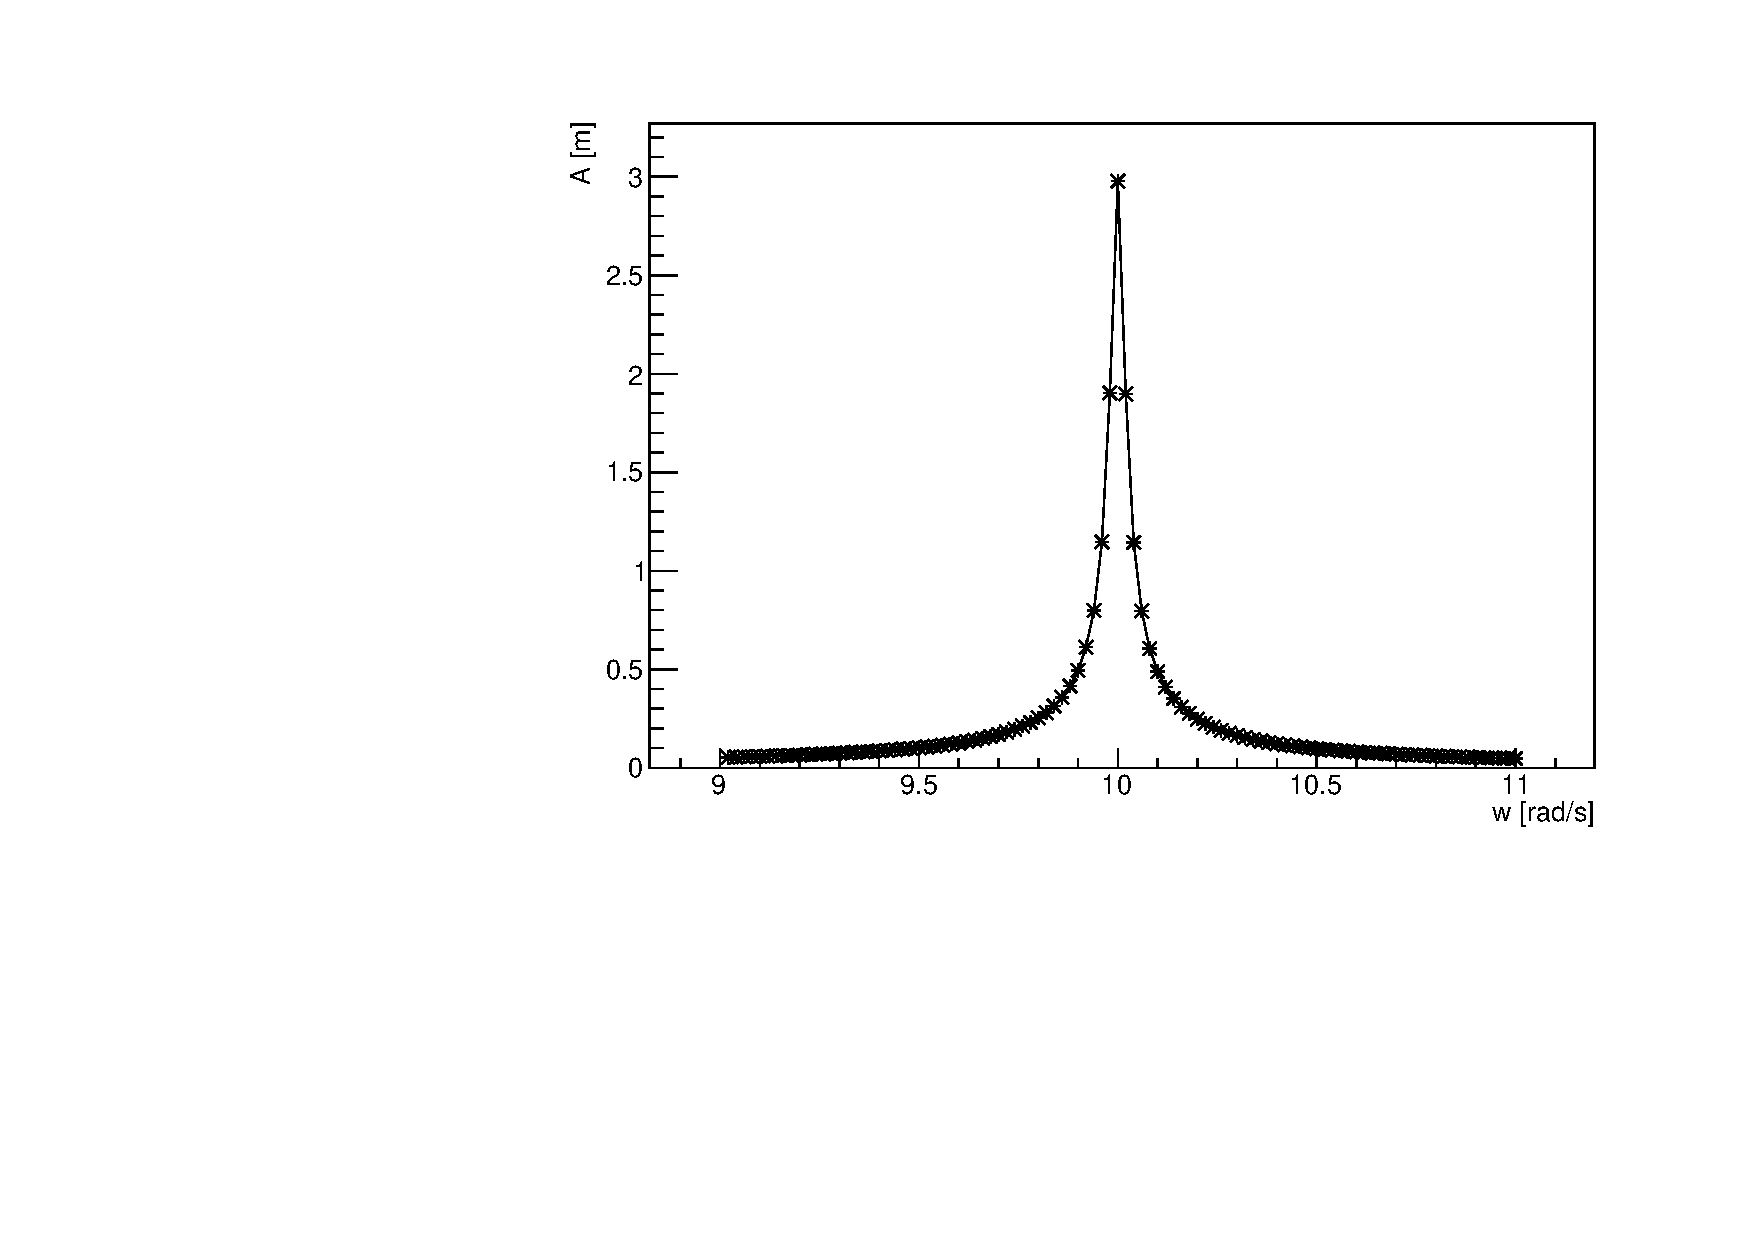
\includegraphics[scale=\scaledim]{Immagini/scatter.pdf}  
	\caption{Plot: una lorentziana}
	\label{root2}
\end{figure}
Un istogramma, invece, è quello in figura \ref{root3}.



\subsection{TH1F}
Per disegnare un istogramma, la libreria da usare è ``TH1F.h''. Vediamo il codice:
\begin{lstlisting}
#include <iostream>
#include "TApplication.h"
#include "TCanvas.h"
#include "TH1F.h"
using namespace std;

int main(){
	TApplication app("app", 0,0);
	TCanvas canvas;
	int n_bin=10; //numero di bin in cui dividere l'istogramma, il numero di ''barre'' dell'istogramma
	float min=3.3, max=6.7; //valore minimo e massimo per l'ascissa dell'istogramma (i ''canali'')
	TH1F histo("Istogramma", "Somme", n_bin, min, max); //nome da far apparire nella tabellina riassuntiva, nome da far apparire in alto, numero di bin, canale minimo e canale massimo
	//...
	//...
	for(int i=0; i<n_punti; ++i)
		histo.fill(v[i]); //v e' un vettore contenente i nostri punti
	canvas.cd(); //seleziono la canvas su cui disegnare
	histo.Draw(); //disegno l'istogramma
	app.Run(); //faccio partire ROOT
	return 0;	
}
\end{lstlisting}
\begin{figure} [h!]
	\centering
	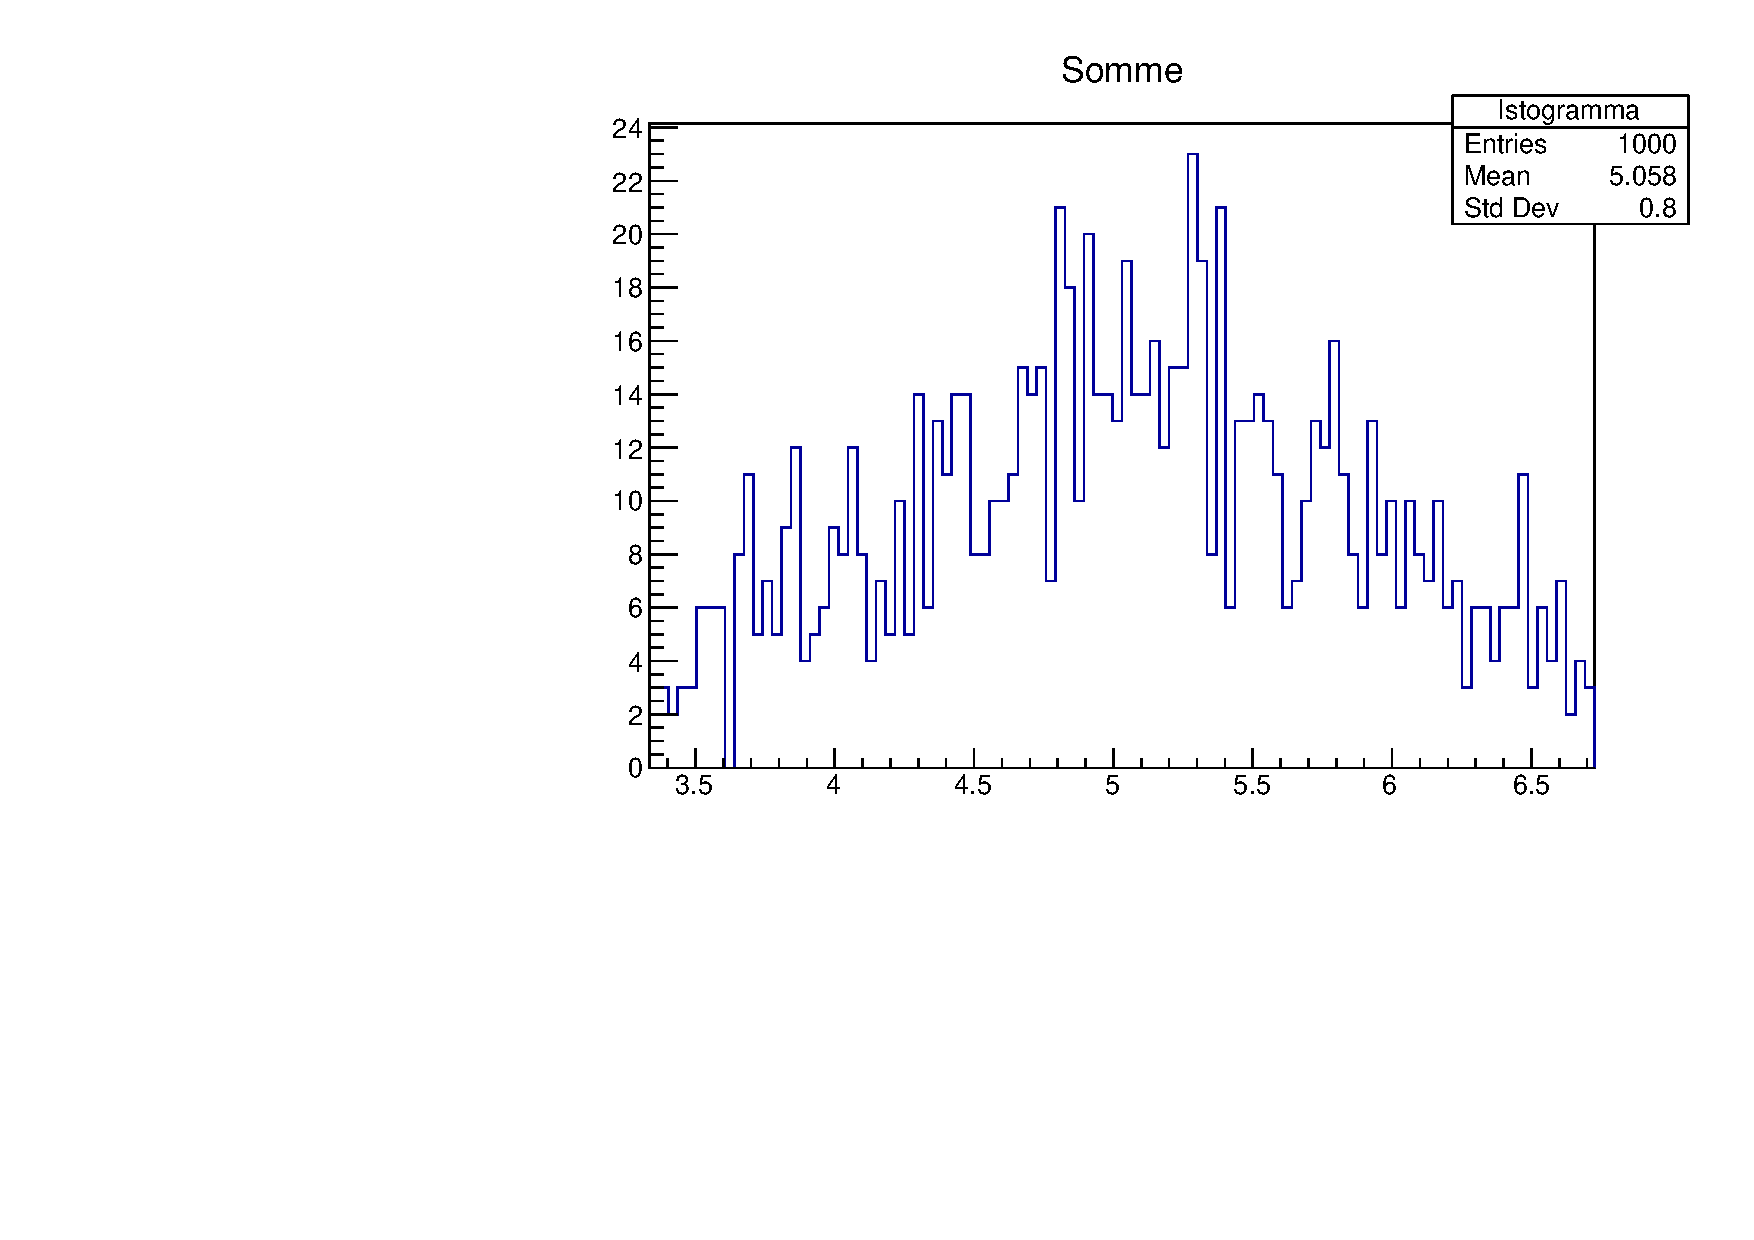
\includegraphics[scale=\scaledim]{Immagini/histo.pdf}  
	\caption{Istogramma}
	\label{root3}
\end{figure}
Quando dichiariamo un oggetto, la classe istogramma vuole come parametri  (tra le tonde) i seguenti elementi: il nome da far apparire nella tabella riassuntiva (in alto a destra della figura \ref{root3}), il nome da far apparire in alto nella canvas (``Somme'' in figura \ref{root3}), il numero di bin in cui suddividere l'istogramma (il numero di barre) e, infine, il valore del bin minimo e massimo (ad esempio, sempre in figura \ref{root3} sono rispettivamente 3.3 e 6.7). A questo punto, riempiamo l'istogramma con i nostri dati tramite il metodo \emph{Fill(\emph{dato\_da\_inserire})}: la classe \emph{TH1F}, da sola, posiziona il dato nel bin corretto e costruisce l'istogramma (sulle ordinate vi è, quindi, il numero di dati per ogni bin).

Infine, dobbiamo selezionare la canvas su cui vogliamo disegnare (possiamo, infatti, avere più canvas nello stesso programma) e, tramite il metodo \emph{Draw()}, stampare l'istograma. Quindi, dobbiamo far ``partire'' l'applet di ROOT con il metodo \emph{Run()} della classe \emph{TApplication}.\\

Un'alternativa consiste nel riempire noi i bin senza lasciare che venga fatto in modo automatico: dobbiamo usare il metodo \emph{SetBinContent(\emph{i, n\_dati})} che permette di inserire n\_dati nell'i-esimo bin (dove i, tanto per uniformarsi al \verb|C++|, parte da 1\ldots). 

Il seguente esempio riempie casualmente i cinque bin di un istogramma, e il risultato è mostrato in figura \ref{root4}:
\begin{lstlisting}
#include <cstdlib>
#include <ctime>
#include "TApplication.h"
#include "TCanvas.h"
#include "TH1F.h"
using namespace std;

int main(){
	TApplication app("app", 0,0);
	TCanvas canvas;
	TH1F histo("Dati", "Istogramma", 5, 0,5); //nome nella tabella dei dati, nome in alto, numero di bin, valore bin minimo, valore bin massimo (in questo caso questi ultimi due valore non servono a niente: siamo noi a riempire)

	srand(time(NULL));    
	for(int i=0; i<5;++i) //riempio ogni bin con un numero di dati casuale
		histo.SetBinContent(i+1, rand()); //i parte da 1
	canvas.cd();
	histo.Draw();
	app.Run();

	return 0;
}
\end{lstlisting}

\begin{figure} [h]
	\centering
	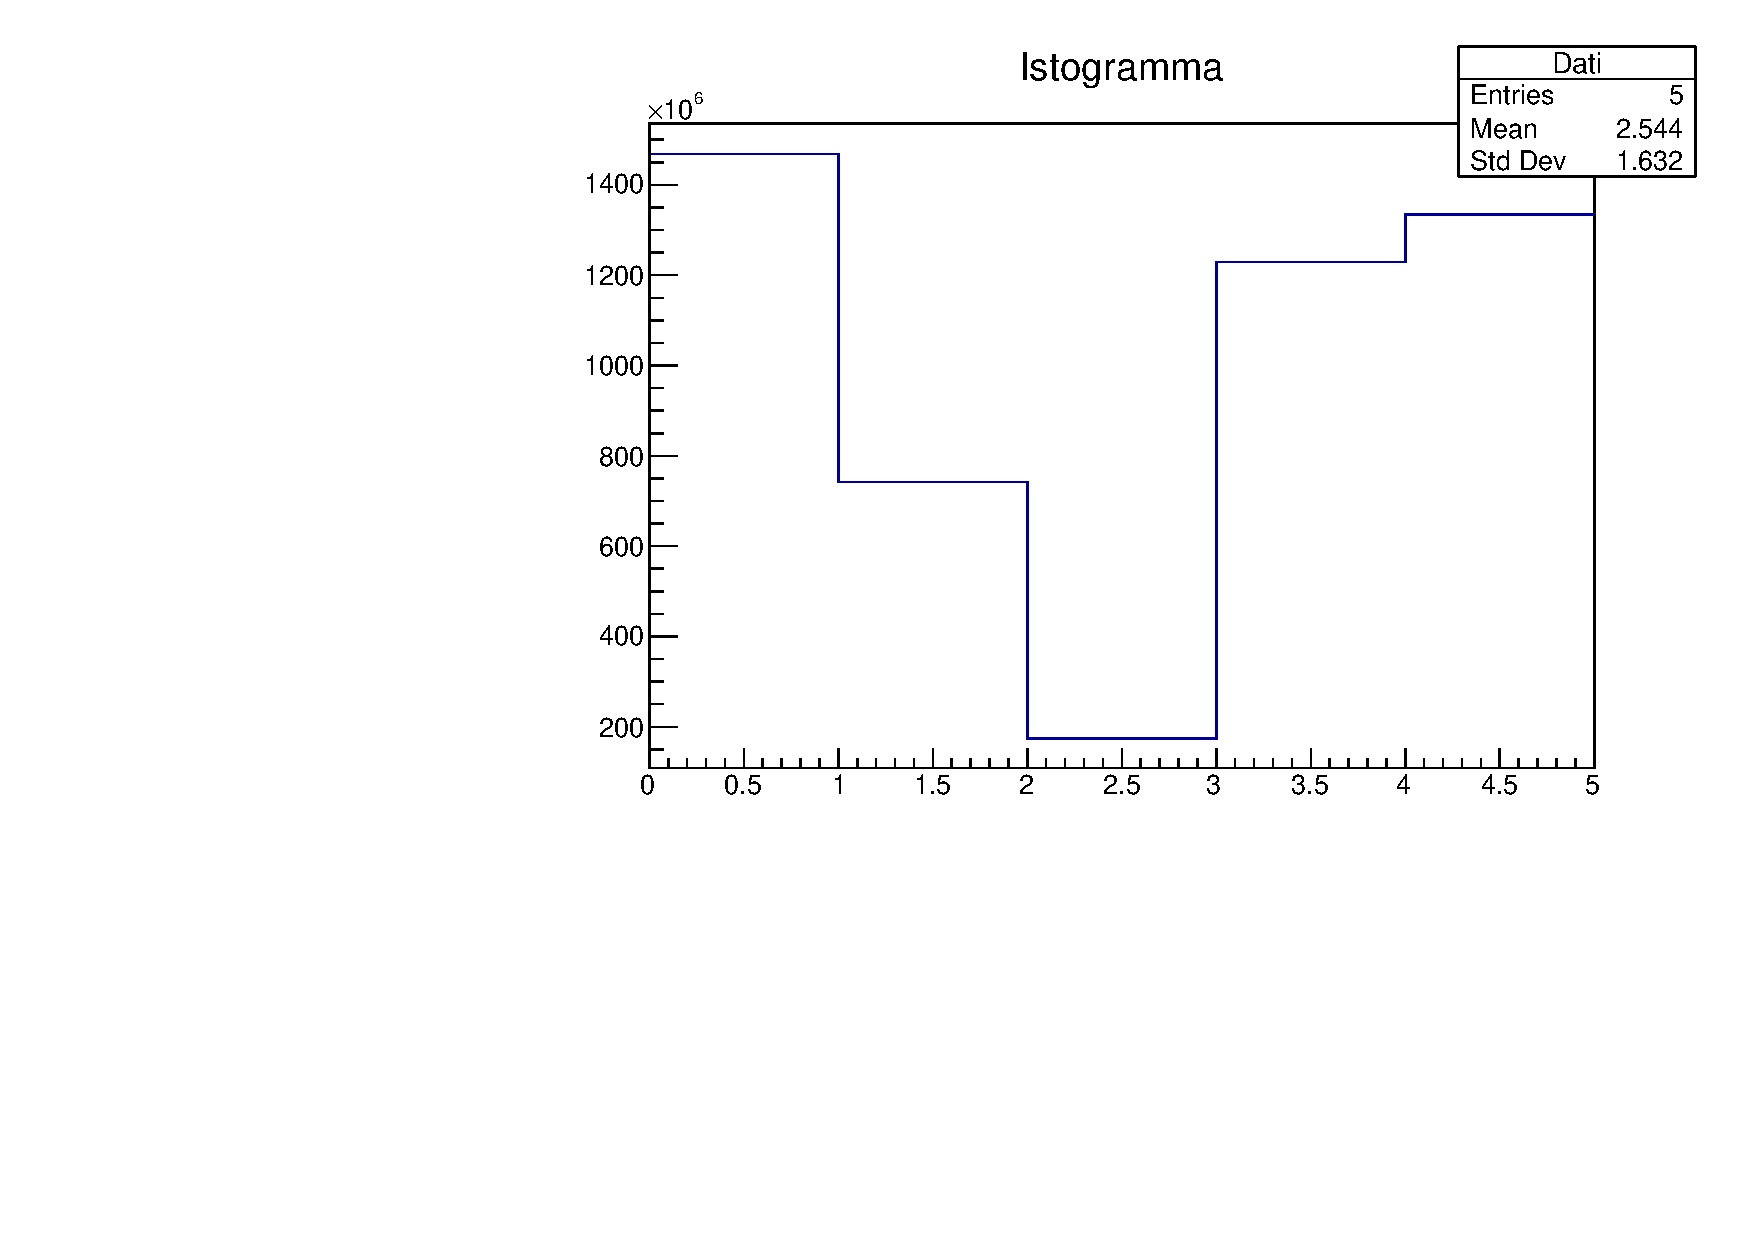
\includegraphics[scale=\scaledim]{Immagini/histo2.pdf}  
	\caption{Istogramma casuale}
	\label{root4}
\end{figure}
Per informazione, la figura all'inizio del capitolo (\ref{root1}) è stata realizzata proprio in questo modo: è stata usata la classe \emph{TH1F} riempiendo manualmente i bin (in ogni bin vi è il numero di particelle che ha colpito il rivelatore a quella data energia). Non si nota che è un istogramma in quanto i bin sono più di ottomila.
\subsection{TGraph}
La classe \emph{TGraph} (contenuta nella libreria \emph{TGraph.h}) permette, invece, di realizzare un plot di dati. Molto semplicemente, si utilizza il metodo \emph{SetPoint(i, x, y)}: i è l'i-esimo punto (che questa volta, invece, parte da zero), x è l'ordinata e y l'ascissa.  Vediamo un esempio. 

Il codice che segue disegna 100 punti con ordinata e ascissa uniformemente distribuite tra 0 e 1:

\begin{lstlisting}[label=esroot1]
#include <cstdlib>
#include <ctime>
#include "TApplication.h"
#include "TCanvas.h"
#include "TGraph.h"
using namespace std;

int main(){
	TApplication app("app", 0,0);
	TCanvas canvas;
	TGraph grafico; 
	srand(time(NULL));    
	for(int i=0; i<100;++i) 
		grafico.SetPoint(i,rand()/(float)RAND_MAX,  rand()/(float)RAND_MAX); //Perche' ho scritto il (float)? Se non lo metto che numeri (o meglio: che numero) vengono generati?
	canvas.cd();
	grafico.Draw("A*"); //quando disegno un grafico devo dargli delle opzioni
	app.Run();
	return 0;
}

\end{lstlisting}
\begin{figure} [ht]
	\centering
	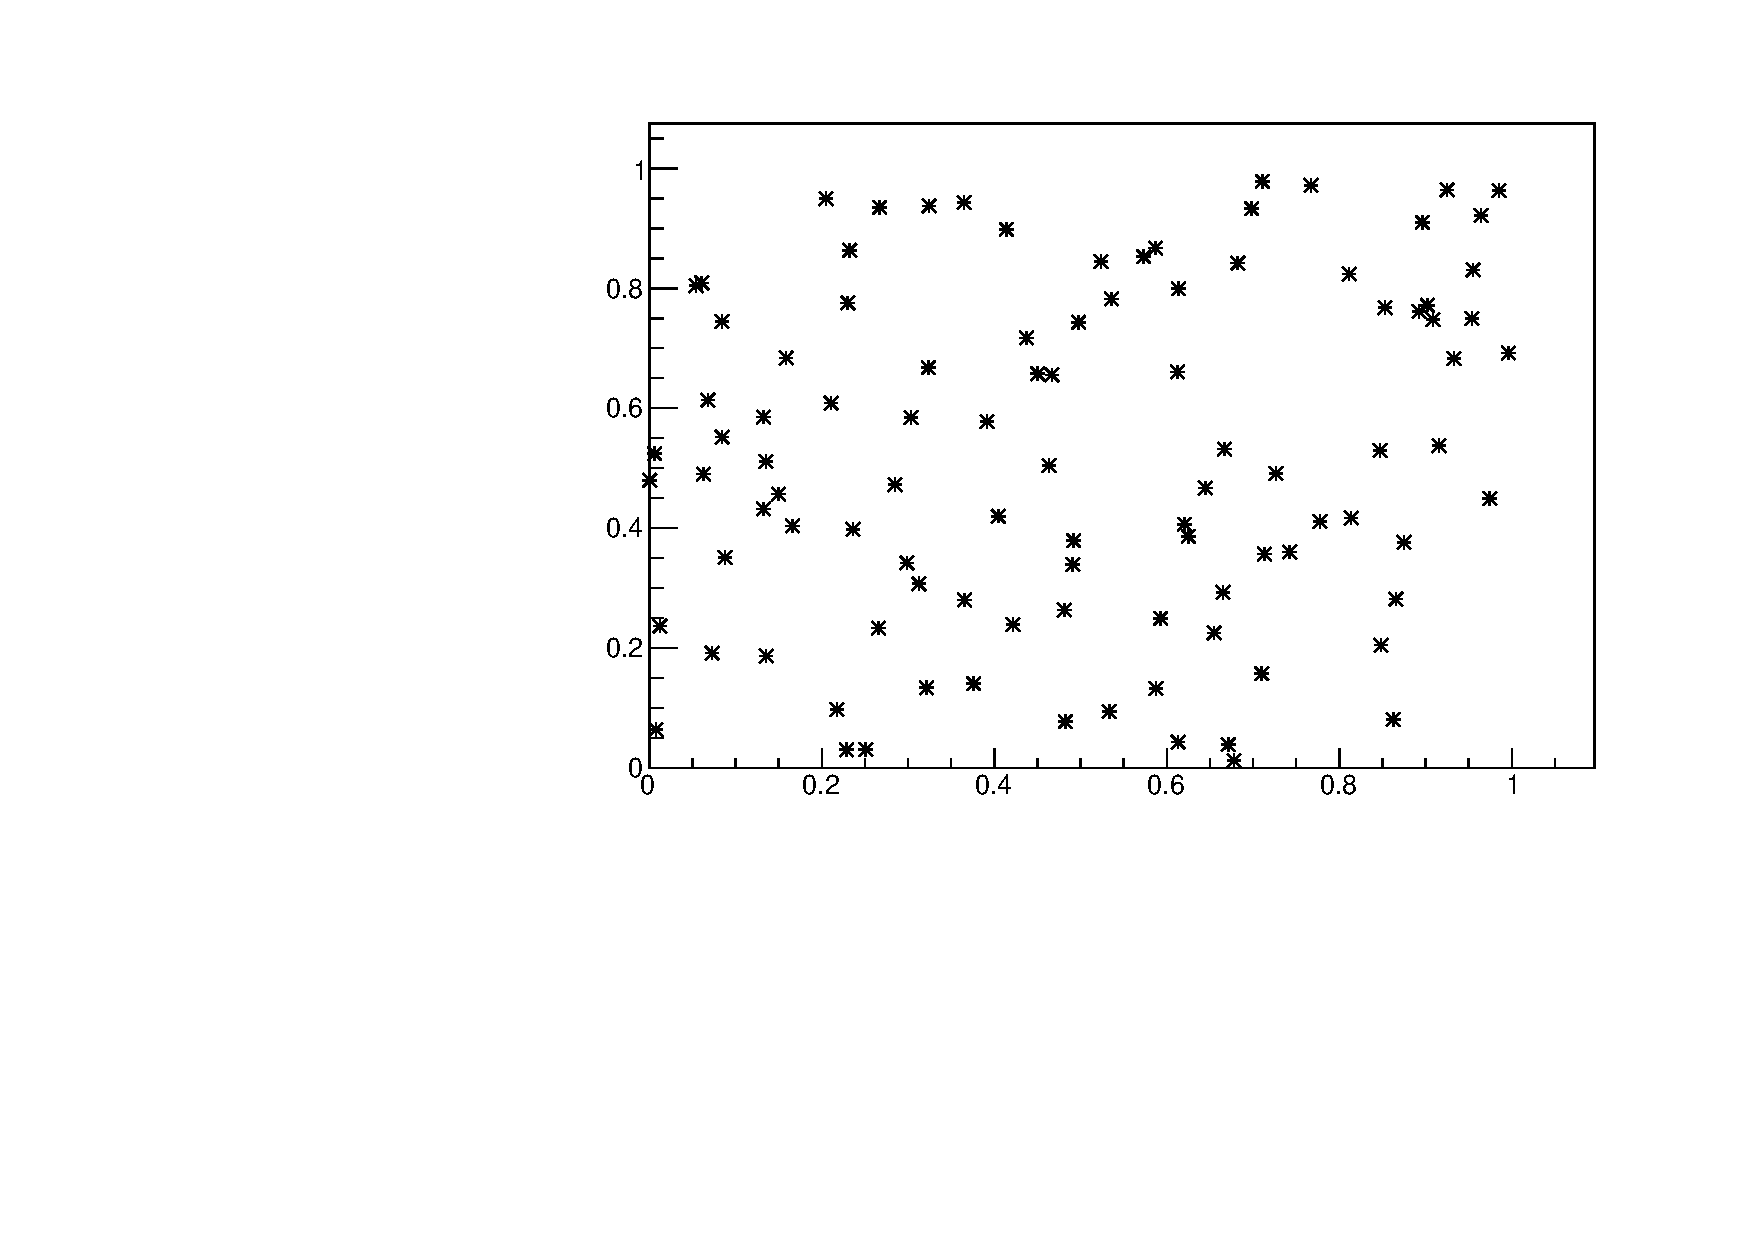
\includegraphics[scale=\scaledim]{Immagini/randomplot.pdf}  
	\caption{Plot di dati random}
	\label{root5}
\end{figure}

L'unica differenza rispetto agli esempi precedenti è questa: quando disegno un grafico devo dire alla classe \emph{TGraph} come rappresentare i punti. Per farlo, si passa una stringa al metodo \emph{Draw}: la ``A'' indica di disegnare gli assi del grafico; l' ``*'' indica di disegnare i punti con degli asterischi. Il grafico in figura \ref{root2} aveva in più l'opzione ``L'' che indica di collegare i punti con una riga continua: infatti, avevo passato la stringa ``AL*''.

Il risultato del codice dell'esempio \ref{esroot1} è la figura \ref{root5}.


\subsection{Nomi degli assi e funzioni}
Potremmo desiderare di mettere grandezze e unità di misura sugli assi. La classe \emph{TGraph} supporta questa funzionalità tramite un metodo che restituisce un oggetto \emph{TAxis}, il quale permette di inserire nomi sugli assi (va inclusa la libreria \emph{TAxis.h}). Vediamo come:
\begin{lstlisting}[label=esroot2]
#include <iostream>
#include "TApplication.h"
#include "TCanvas.h"
#include "TGraph.h"
#include "TCanvas.h"
#include "TAxis.h"
using namespace std;

int main(){
	TApplication app("app", 0,0);
	TCanvas canvas;
	TGraph grapico;
	
	//riempio il grafico
	//...
	//...
	
	canvas.cd();
	grafico.GetXaxis()->SetTitle("V [V]"); //Nome all'asse X
	punti.GetYaxis()->SetTitle("I [mA]"); //Nome all'asse Y
	grafico.Draw("A*");
	app.Run();
	return 0;
	
}
\end{lstlisting}

L'esempio \ref{esroot2} permette di dare i nomi agli assi come in figura \ref{root6}. Da notare cosa ho scritto: si accede al metodo \emph{GetXaxis()} (o Y) dell'oggetto \emph{TGraph}. Questo, quindi, restituisce un puntatore ad un oggetto della classe \emph{TAxis}: perciò, dobbiamo usare l'operatore ``->'' per accedere al metodo \emph{SetTitle("nome")}.

L'ultima cosa che ci rimane da imparare è disegnare una funzione matematica sopra ad un grafico. La questione è piuttosto semplice: si utilizza la classe \emph{TF1} contenuta nella libreria \emph{TF1.h}. Ecco un esempio:

\begin{lstlisting}[label=esroot2]
#include <iostream>
#include "TApplication.h"
#include "TCanvas.h"
#include "TGraph.h"
#include "TCanvas.h"
#include "TAxis.h"
#include "TF1.h"
using namespace std;

int main(){
	TApplication app("app", 0,0);
	TCanvas canvas;
	TGraph grapico;

	//riempio il grafico
	//...	
	//...

	canvas.cd();
	grafico.GetXaxis()->SetTitle("V [V]"); 
	punti.GetYaxis()->SetTitle("I [mA]"); 
	grafico.Draw("A*");

	//Funzone retta
	TF1 retta("Retta", "[0]*x+[1]",min , max); //in ordine: nome, formula parametrica, definita tra minimo e massimo
	float m=10.;
	float q=0.;	
	retta.SetParameter(0, m); //assegno valore al parametro "[0]" 
	retta.SetParameter(1, q); //assegno valore al parametro "[1]"
	retta.Draw("SAMEL"); //SAME sta per sulla stessa canvas selezionata prima, sopra al grafico, L per usa una linea
	app.Run();
	return 0;
}
\end{lstlisting}
\begin{figure} [ht]
	\centering
	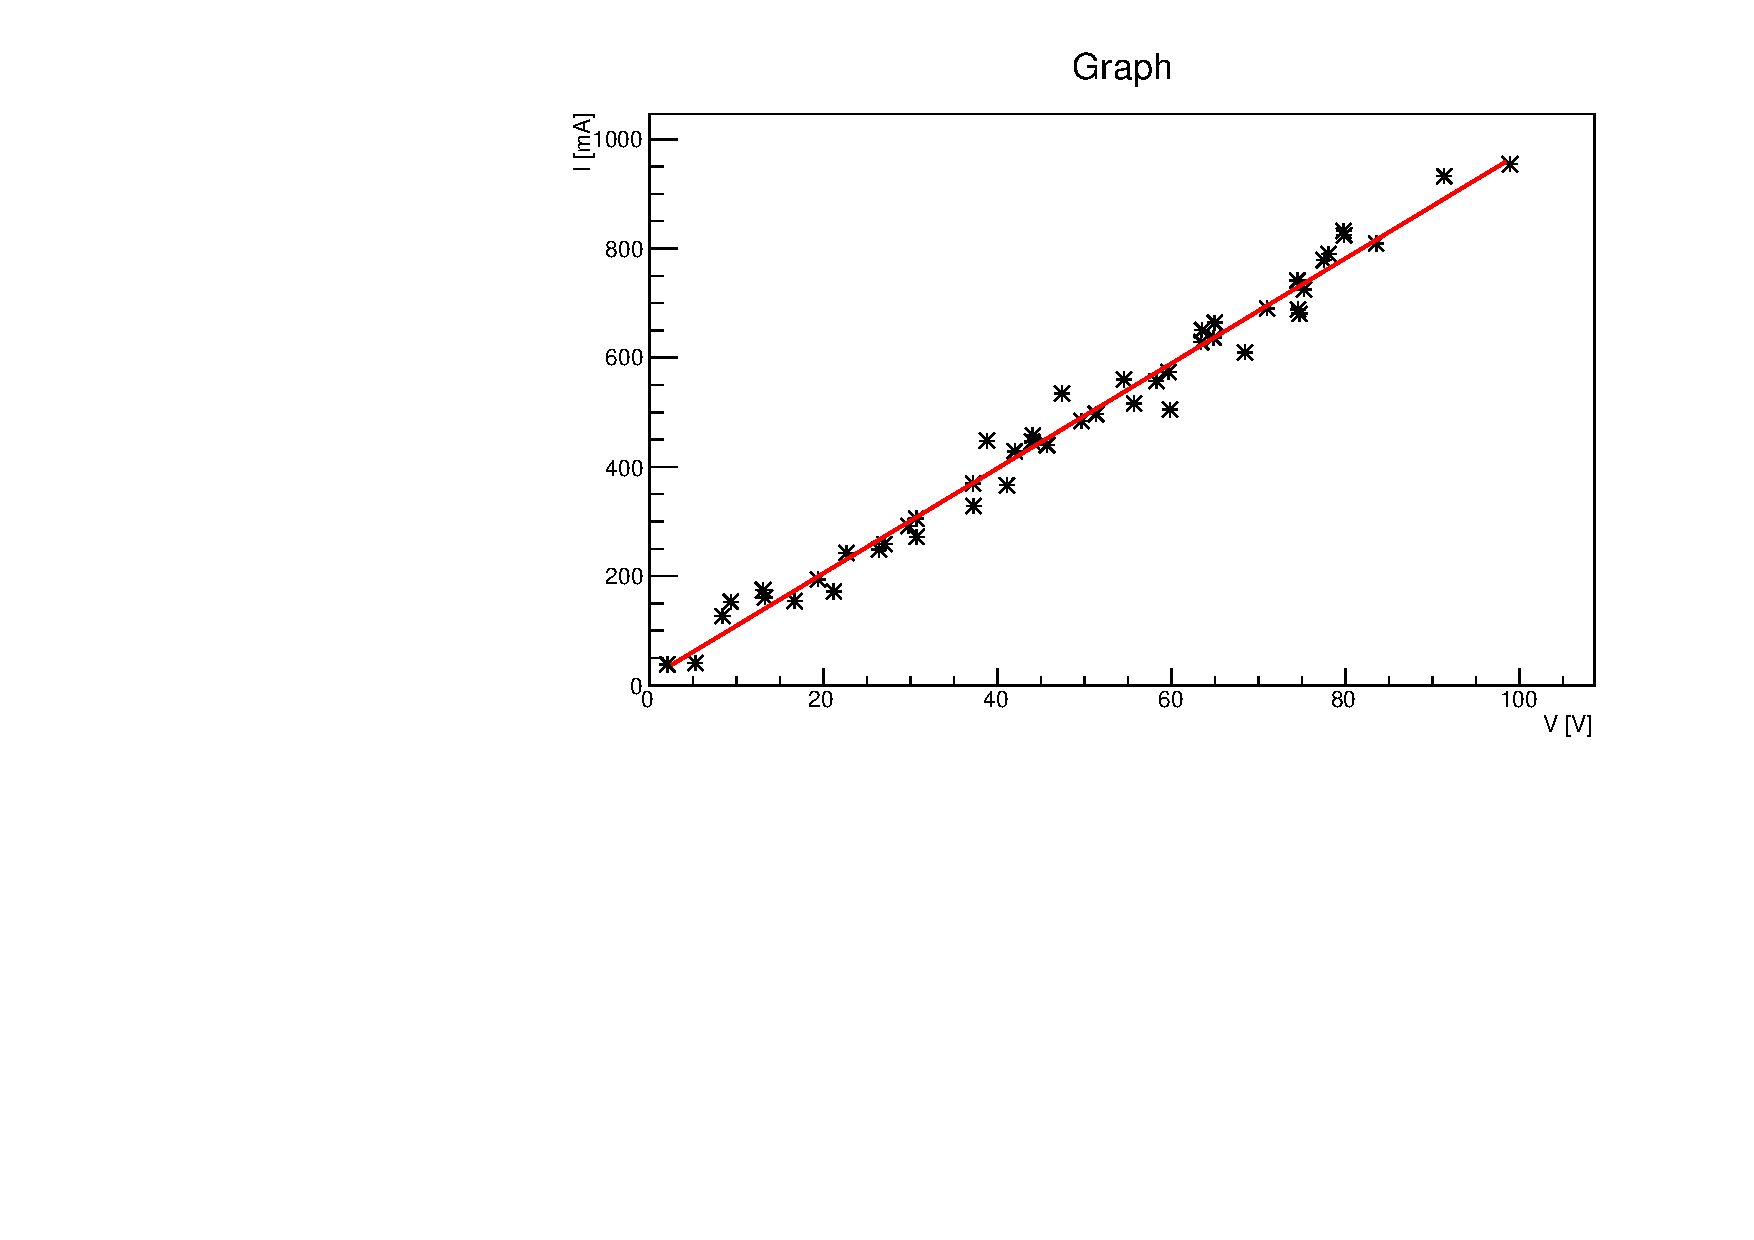
\includegraphics[scale=\scaledim]{Immagini/retta.pdf}  
	\caption{Fit lineare}
	\label{root6}
\end{figure}



ROOT, oltre alle funzioni analizzate, ha tante altre caratteristiche. Se vai sul sito di ROOT  e accedi alla reference (\url{https://root.cern.ch/documentation}), puoi trovare informazioni su tutto quello che è disponibile e su come usarlo. Va detto che la reference di ROOT non è eccellente e spesso è davvero difficoltoso capire come utilizzare i suoi strumenti.
\subsubsection{Una nota conclusiva su ROOT}
ROOT non è l'unica soluzione che permette di affrontare le problematiche del plot di dati, disegnare funzioni, analisi dati, ecc\ldots A dirla tutta, vi sono linguaggi orientati esclusivamente a queste finalità, alcuni molto semplici da utilizzare. 

Per l'analisi dati, ad esempio, \emph{Matlab} e  \emph{Octave} possono risultare molto più potenti, efficaci e facili da usare (i fit, anche delle funzioni più esotiche, si realizzano in qualche di riga di codice). Un linguaggio di programmazione di livello più alto del \verb|C++| che dispone di bellissime librerie orientate al calcolo scientifico è \emph{Python} (librerie utilissime sono \emph{matplotlib}, \emph{scipy} e \emph{numpy}). Se, invece, devi solo plottare dati o graficare funzioni (facendo, magari, qualche fit) il leggerissimo e semplice programma \emph{Gnuplot} può essere una soluzione valida. Se, al contrario, vuoi usare il computer per risolvere problemi di Analisi matematica, Geometria, ecc\ldots, magari in maniera analitica e non numerica, sapere dell'esistenza di \emph{Mathematica} (purtroppo non free) potrebbe esserti molto utile.

Ovviamente non sto insinuando che tu debba impararti tutti questi linguaggi ma, se ti intriga conoscere strumenti diversi, perché non dare un'occhiata? Il vantaggio di conoscere più linguaggi è di saper scegliere, di fronte ad un problema, quello che porta alla soluzione in maniera più rapida, efficiente e comoda. 